\begin{frame}
    \frametitle{Reinforcement Learning\footfullcite{sutton2018reinforcement}}
    \begin{figure}
        \centering
        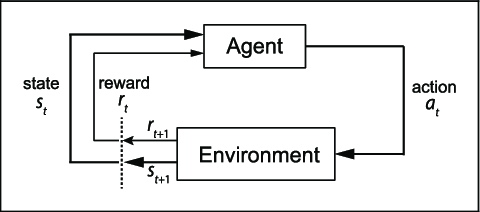
\includegraphics[height=0.3\textheight]{figs/rl.png}
    \end{figure}
\end{frame}

\begin{frame}
    \frametitle{Multi armed bandit (Chp 2)}
    \begin{itemize}
        \item Stateless, tradeoff between exploration and exploitation.
        \item Action value function $Q_t(a)$: at time $t$, action $a$'s expected reward.
        \item Solutions:
              \begin{itemize}
                  \item $\epsilon$-greedy: give $\epsilon$ chance of random selection(exploration), otherwise greedily chose best arm(exploitation) (Chp 2.3)
                  \item Upper-Confidence-Bound (Used in last paper we discussed\footfullcite{wangreinforcement}) (Chp 2.7)
              \end{itemize}
    \end{itemize}
\end{frame}

\begin{frame}
    \frametitle{Markov Desicion Process (Chp 3)}
    \begin{itemize}
        \item ``The reward signal is your way of communicating to the robot \textit{what} you want it to achieve, not \textit{how} you want it achieved.''
        \item ``In general, actions can be any decisions we want to learn how to make, and the states can be anything we can know that might be useful in making them.''
        \item Policy: a distribution of actions to take. $\pi(a|s)$: Given current state $s$, the probablity of selecting action $a$.
        \item State function: $v_\pi(s)$: given policy $\pi$, how good are we to be at state $s$?
        \item We want to find the best \textbf{espected return}, so it's not really greedy.
        \item Discount history reward for math and engineering reasons:
              \begin{itemize}
                  \item Avoid infinite amount when $t\rightarrow\infty$.
                  \item History may not reflect the future, e.g., a fuzzed seed may not generate the same reward it used to.
              \end{itemize}
    \end{itemize}
\end{frame}

\begin{frame}
    \frametitle{Suppose we have a perfect model... Dynamic Programming (Chp 4)}
    \begin{itemize}
        \item We have a perfect model, i.e. we don't need to interact with the environment to know the reward, $v_\pi(s)$ can be computed in Formula 4.4.
        \item Start with a random policy, iteratively update value function, then derive a new policy (Example 4.1).
        \item Generalized Policy Iteration(GPI) (Sec 4.4)
    \end{itemize}
\end{frame}

\begin{frame}
    \frametitle{We don't really have a model... Monte Carlo Methods (Chp 5)}
    \begin{itemize}
        \item Problem is too complicated(fuzzing), or simple problem with hard model(Blackjack)
        \item $v_\pi(s)$ is not good enough, since most states can't be fully experimented, therefore we work on $q_\pi(s, a)$.
        \item Each game is an episode, finish an episode and reversely update $q_\pi(s, a)$.
              \begin{itemize}
                  \item On-policy: Explore the episode with our derived policy, but how do we explore? Exploring start(Chp 5.3) or $\epsilon$-greedy (Chp 5.4).
                  \item Off-policy: Explore the episode using another policy, but how to reflect the reward on our policy? Importance Sampling (Chp 5.5)
              \end{itemize}
    \end{itemize}
\end{frame}

\begin{frame}
    \frametitle{We don't want to finish a game too... Temperal Difference (Chp 5, 6)}
    \begin{itemize}
        \item Can be implemented online (compared to Monte Carlo), doesn't need a model (compared to DP)
        \item Immediately update $v_\pi(s)$ after a step. (Formula 6.2):
              \begin{itemize}
                  \item On-policy SARSA: Update based on the \textbf{next} state-action pair. (Formula 6.7)
                  \item Off-policy Q-learning: Update based on the \textbf{best} state-action pair. (Formula 6.8)
              \end{itemize}
        \item Chp 7: n-step bootstrapping. Tradeoff between TD and monte Carlo, update based on next n steps.
    \end{itemize}
\end{frame}

\begin{frame}
    \frametitle{Tabular method and approximate solution}
    \begin{itemize}
        \item Tabular: You can write state-action pair in a table and update each entry based on your experience.
        \item If the table is too large, i.e. too many states, you have to approximate a state value using known info.
        \item Gradient policy method directly approximates the policy.
    \end{itemize}
\end{frame}

\begin{frame}
    \frametitle{Gradient policy method\footfullcite{sutton1999policy}}
    \begin{itemize}
        \item Policy is parameterizxed by $\mathbf{\theta}$, i.e. $\pi(a|s,\mathbf{\theta})$.
        \item $\mathbf{\theta}$ can be a lot of things. For example, it can ba all weights of a deep artifical neural network.
        \item Performance measure $J(\mathbf{\theta}) = v_{\pi_\mathbf{\theta}}(s_0)$, i.e. how good is the initial state?
        \item Policy gradient theorem makes $\nabla J$ computable (Chp 13.2)
    \end{itemize}
\end{frame}